\documentclass{jsarticle}
\usepackage[dvipdfmx]{graphicx}
\usepackage{bm}
\usepackage{amsmath}
\usepackage{amssymb}
\usepackage{amsfonts}
\usepackage{comment}
\usepackage{listings}
\usepackage{cases}
\lstset{
    basicstyle={\ttfamily},
    identifierstyle={\small},
    commentstyle={\smallitshape},
    keywordstyle={\small\bfseries},
    ndkeywordstyle={\small},
    stringstyle={\small\ttfamily},
    frame={tb},
    breaklines=true,
    columns=[l]{fullflexible},
    numbers=left,
    xrightmargin=0zw,
    xleftmargin=3zw,
    numberstyle={\scriptsize},
    stepnumber=1,
    numbersep=1zw,
    lineskip=-0.5ex,
    keepspaces=true,
    language=c
}
\renewcommand{\lstlistingname}{リスト}
\makeatletter
\newcommand{\figcaption}[1]{\def\@captype{figure}\caption{#1}}
\newcommand{\tblcaption}[1]{\def\@captype{table}\caption{#1}}
\makeatother

\title{プログラミング演習$\rm I\hspace{-.01em}I$課題レポート}
\author{Ec5 24番 平田 蓮}
\date{}

\begin{document}
\maketitle
\section*{課題$\rm I$}
    \subsection*{1.}
        \begin{description}
            \item[grep]{
                ファイル内の文字列を検索するコマンド。\cite{grep} \\
                用例: \verb|grep 検索対象の文字列 検索するファイル| \\
                テキスト\cite{text}のリスト6から``\verb|glVertex|''
                を検索した結果をリスト\ref{src:grep}に示す。
            }
            \item[touch]{
                ファイルのタイムスタンプを書き換えるコマンド。\cite{touch} \\
                用例: \verb|touch オプション ファイル名| \\
                オプションを指定しない場合、
                指定したファイルのタイムスタンプが現在に更新される。
                また、指定したファイルが存在しない場合、
                ファイルを新規作成する。
                一般的にはこの機能を用いて、新規ファイルを作成するコマンドとして用いられる。
                オプションを以下に示す。
                \begin{description}
                    \item[-d] 日時を指定する。
                    \item[-c] ファイルの作成を行わない。
                    \item[-r] 指定したファイルのタイムスタンプを別のファイルのそれとあわせる。
                \end{description}
            }
        \end{description}
        \begin{lstlisting}[caption=grepコマンドの出力, label=src:grep]
    glVertex2d(0, 1);
    glVertex2d(0, 0);
    glVertex2d(1, 0);\end{lstlisting}

    \subsection*{2.}
        \begin{description}
            \item[有効範囲]{
                C言語のソースコードにおいて、\verb|{}|で囲まれた範囲のことを有効範囲と呼ぶ。
                変数は、自身が宣言された有効範囲内でのみ使用することができる。
                特にソースコードの一番外側の有効範囲(\verb|main()|の外側)
                で宣言された変数はグローバル変数と呼ぶ。
            }
            \item[記憶期間]{
                C言語において変数宣言をする際は、
                \verb|auto|, \verb|static|などのキーワードを用いることができる。
                (用例:\verb|auto int a=100;static double b=4.6;|)
                デフォルト値は\verb|auto|で、これは省略可能である。
                \verb|auto|を使用して宣言された変数は自動記憶域期間を持つ。
                これはプログラムが実行される中で記述通りのタイミングで生成され、
                有効範囲の実行が完了した時点で遺棄される。
                また、初期値の指定がない場合は不定値となる。
                一方\verb|static|を使用すると変数は静的記憶域期間を持つ。
                これはプログラムの開始時に生成され、
                プログラムの終了時まで保持される。
                さらに、初期値が指定されない場合は自動的に0で初期化される。
            }
        \end{description}

    \subsection*{3.}
        プログラムを一部抜粋してリスト\ref{src:star}に示す。

        \begin{lstlisting}[caption=星型正多角形を描くプログラム, label=src:star]
#define VERTEX_NUM 7
#define ROTATION_SPEED M_PI / 50.0

void display() {
    static double rotation, dt = 4.0 * M_PI / (double)VERTEX_NUM;
    double x, y, theta = rotation;
    int i;
    
    glClear(GL_COLOR_BUFFER_BIT);

    glColor3d(0, 0, 0);

    glBegin(GL_LINES);
    for (i = 0; i < VERTEX_NUM * 2; i++, theta += dt) {
        x = cos(theta);
        y = sin(theta);

        glVertex2d(x, y);
    }

    glEnd();
    glutSwapBuffers();

    rotation += ROTATION_SPEED;
}\end{lstlisting}

        \verb|VERTEX_NUM|, \verb|ROTATION_SPEED|はそれぞれ頂点数、回転速度である。
        頂点を一つ飛ばしに結ぶことで図形を描いている。

    \subsection*{4.}
        プログラムを一部抜粋してリスト\ref{src:graph}に示す。

        \begin{lstlisting}[caption=完全グラフを描くプログラム, label=src:graph]
#define VERTEX_NUM 7
#define ROTATION_SPEED M_PI / 50.0

void display() {
    static double rotation;
    double x, y, theta, dt;
    int i, j;
    
    glClear(GL_COLOR_BUFFER_BIT);

    glColor3d(0, 0, 0);

    glBegin(GL_LINES);
    for (i = 1, theta = rotation; i < (double)VERTEX_NUM / 2.0; i++) {
        dt = 2.0 * i * M_PI / (double)VERTEX_NUM;
        for (j = 0; j < VERTEX_NUM * 2; j++, theta += dt) {
            x = cos(theta);
            y = sin(theta);

            glVertex2d(x, y);
        }
    }

    glEnd();
    glutSwapBuffers();

    rotation += ROTATION_SPEED;
}\end{lstlisting}

        星型正多角形は頂点を一つ飛ばしで結んだが、
        0個飛ばしから頂点数の半分個飛ばしまでそれぞれでできる図形を重ねることで
        完全グラフが描ける。

    \subsection*{5.}
        それぞれの図形を描画するプログラムをリスト
        \ref{src:cardioid}, \ref{src:cycloid}, \ref{src:hypocycloid}に示す。

        \begin{lstlisting}[caption=カージオイドを描くプログラム, label=src:cardioid]
void drawAxis() {
    double x, y;

    glBegin(GL_LINES);
    glVertex2d(-0.5, 0);
    glVertex2d(3, 0);
    glVertex2d(0, -1.5);
    glVertex2d(0, 1.5);
    for (x = 0; x < 3; x++) {
        glVertex2d(x, -0.05);
        glVertex2d(x, 0.05);
    }
    for (y = -1; y < 1.5; y += 0.5) {
        glVertex2d(-0.05, y);
        glVertex2d(0.05, y);
    }
    glEnd();
}

void drawCardioid() {
    double x, y, theta;

    glBegin(GL_LINE_STRIP);
    for (theta = 0; theta < 2 * M_PI; theta += 0.01) {
        x = cos(theta) * (1 + cos(theta));
        y = sin(theta) * (1 + cos(theta));

        glVertex2d(x, y);
    }
    glEnd();
}

void display() {
    glClear(GL_COLOR_BUFFER_BIT);

    glColor3d(0, 0, 0);

    drawAxis();
    drawCardioid();

    glutSwapBuffers();
}\end{lstlisting}

        \begin{lstlisting}[caption=サイクロイドを描くプログラム, label=src:cycloid]
void drawAxis() {
    double x, y;

    glBegin(GL_LINES);
    glVertex2d(-0.5, 0);
    glVertex2d(2 * M_PI + 0.5, 0);
    glVertex2d(0, -0.5);
    glVertex2d(0, 2.5);
    for (x = 0; x < 2.5; x += 0.5) {
        glVertex2d(x * M_PI, -0.05);
        glVertex2d(x * M_PI, 0.05);
    }
    for (y = 0; y < 3; y ++) {
        glVertex2d(-0.05, y);
        glVertex2d(0.05, y);
    }
    glEnd();
}

void drawCycloid() {
    double x, y, theta;

    glBegin(GL_LINE_STRIP);
    for (theta = 0; theta < 2 * M_PI; theta += 0.01) {
        x = theta - sin(theta);
        y = 1 - cos(theta);

        glVertex2d(x, y);
    }
    glEnd();
}

void display() {
    glClear(GL_COLOR_BUFFER_BIT);

    glColor3d(0, 0, 0);

    drawAxis();
    drawCycloid();

    glutSwapBuffers();
}\end{lstlisting}

        \begin{lstlisting}[caption=4尖点の内サイクロイドを描くプログラム, label=src:hypocycloid]
void drawAxis() {
    double x, y;

    glBegin(GL_LINES);
    glVertex2d(-1.5, 0);
    glVertex2d(1.5, 0);
    glVertex2d(0, -1.5);
    glVertex2d(0, 1.5);
    for (x = -1; x < 1.5; x += 0.5) {
        glVertex2d(x, -0.05);
        glVertex2d(x, 0.05);
        
        y = x;
        glVertex2d(-0.05, y);
        glVertex2d(0.05, y);
    }
    glEnd();
}

void drawHypocycloid() {
    double x, y, theta;

    glBegin(GL_LINE_STRIP);
    for (theta = 0; theta < 2 * M_PI; theta += 0.01) {
        x = cos(theta);
        x = x * x * x;
        y = sin(theta);
        y = y * y * y;

        glVertex2d(x, y);
    }
    glEnd();
}

void display() {
    glClear(GL_COLOR_BUFFER_BIT);

    glColor3d(0, 0, 0);

    drawAxis();
    drawHypocycloid();

    glutSwapBuffers();
}\end{lstlisting}

        描画結果を図\ref{fig:cardioid}, \ref{fig:hypocycloid}, \ref{fig:cycloid}に示す。

        \begin{figure}[h]
            \begin{minipage}{0.5\hsize}
                \centering
                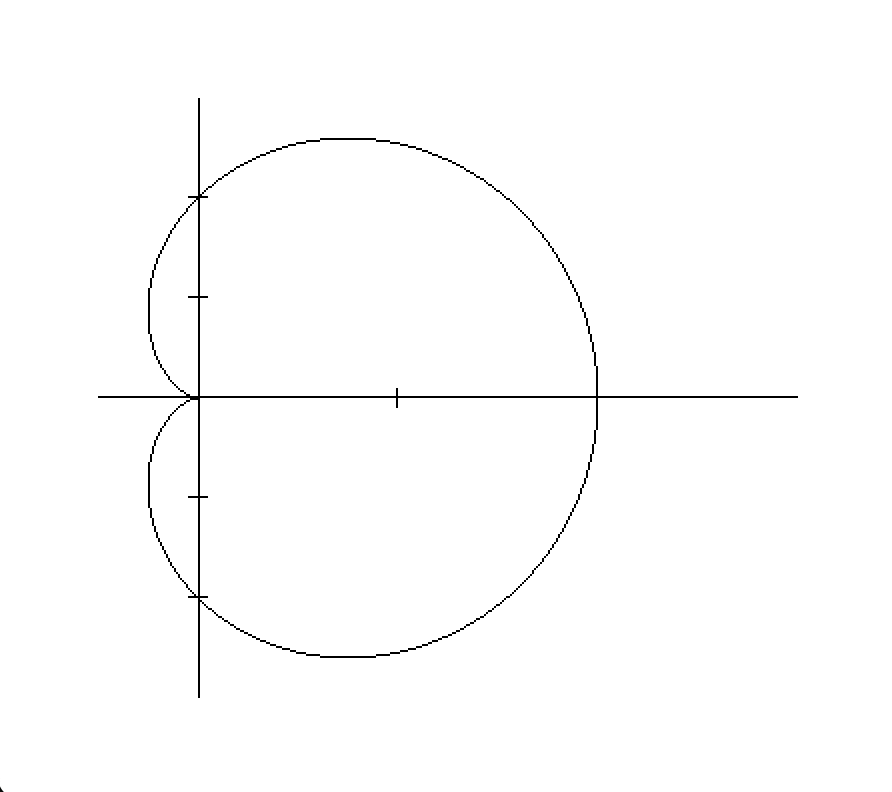
\includegraphics[width=1\hsize]{cardioid.png}
                \caption{カージオイド}
                \label{fig:cardioid}
            \end{minipage}
            \begin{minipage}{0.5\hsize}
                \centering
                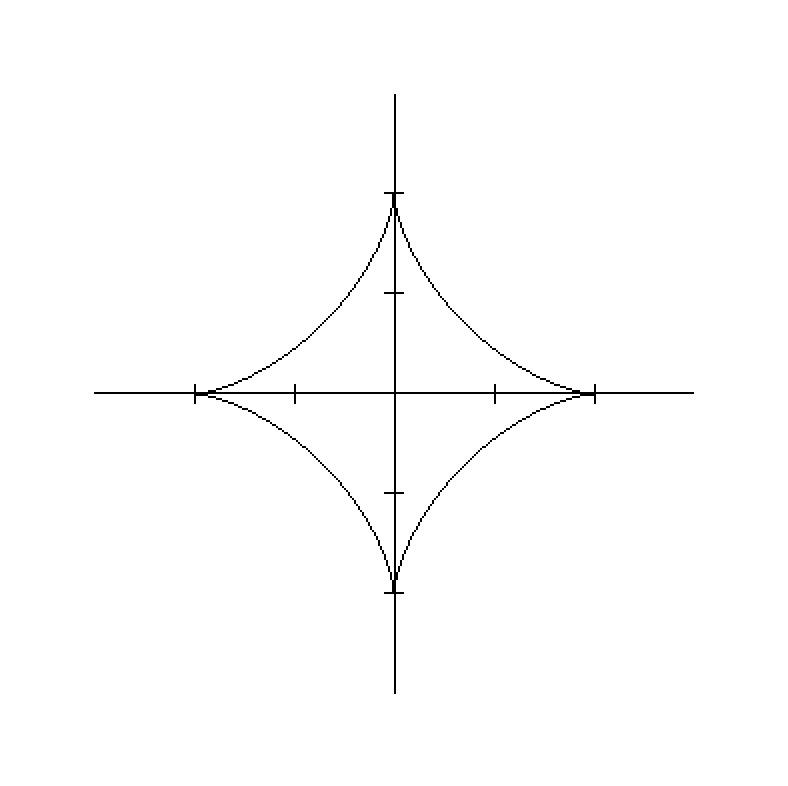
\includegraphics[width=1\hsize]{hypocycloid.png}
                \caption{4尖点の内サイクロイド}
                \label{fig:hypocycloid}
            \end{minipage}
        \end{figure}
        \begin{figure}[h]
            \centering
            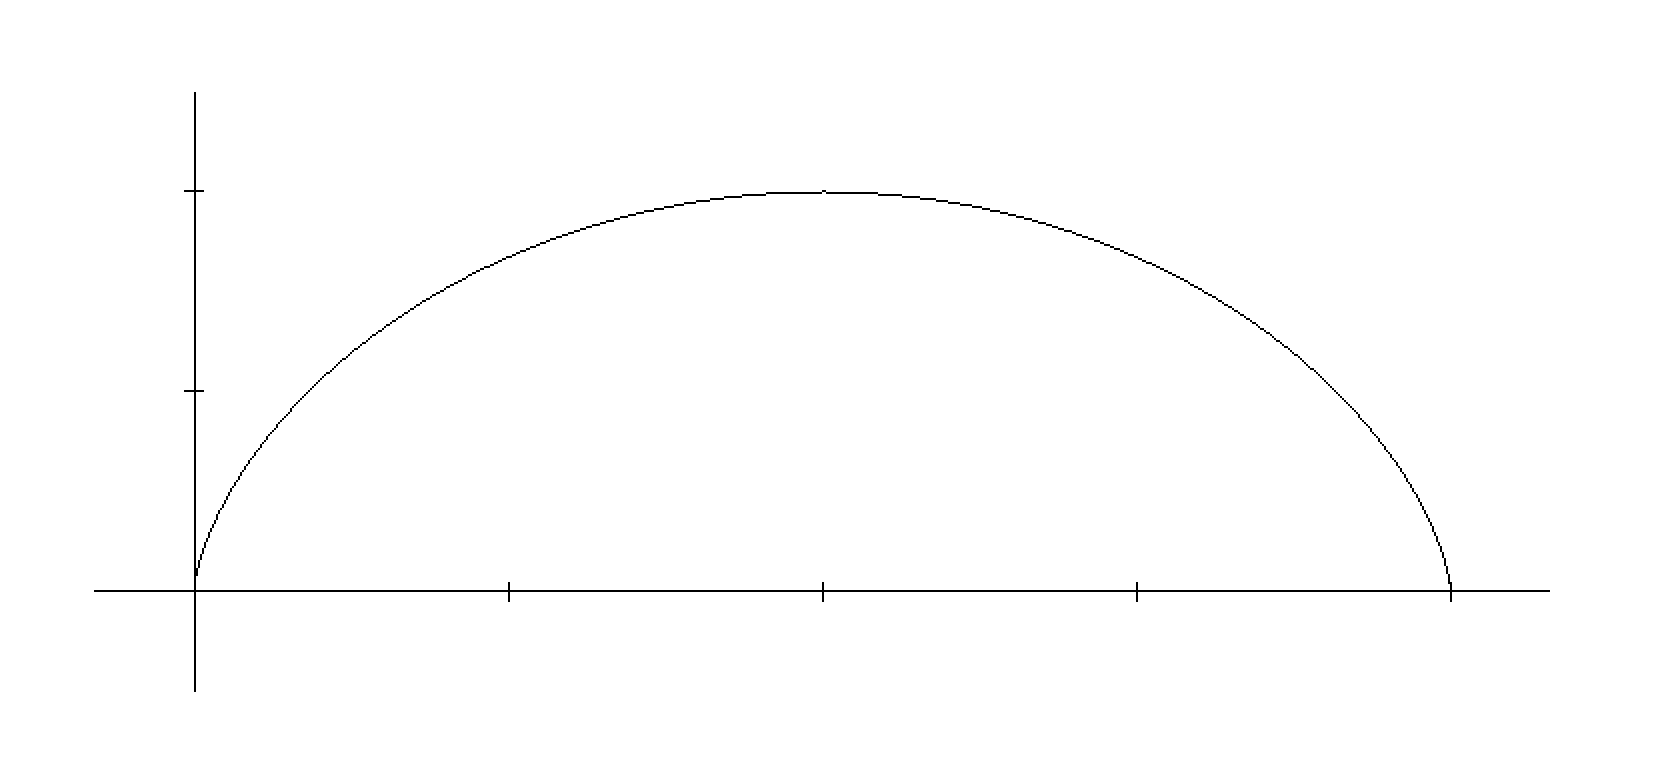
\includegraphics[width=1\hsize]{cycloid.png}
            \caption{サイクロイド}
            \label{fig:cycloid}
        \end{figure}

\section*{課題$\rm I\hspace{-.01em}I$}
    \subsection*{1.}
        $\triangle BGI$に注目すると、$\displaystyle\angle GBI=\frac{\pi}{3}, BI= \frac{w}{2}$
        なので、$\displaystyle GB = \frac{w}{\sqrt{3}}, GI = \frac{w}{2\sqrt{3}}$である。
        同様に、$\displaystyle GH=\frac{w}{2\sqrt{3}}, HC=HD=\frac{w}{2}$である。

        また、正四面体状での$\triangle AGI$に注目すると、三平方の定理より、
        \begin{equation*}
            GA = \sqrt{(AI)^2 - (GI)^2} = \sqrt{(GI + GB)^2-(GI)^2}=\sqrt{\frac{2}{3}}w
        \end{equation*}
        となる。
        
        以上により、各頂点の座標は、
        \begin{equation*}
            A=\left(\sqrt{\frac{2}{3}}w,0,0\right),
            B=\left(0,\frac{w}{\sqrt{3}},0\right),
            C=\left(0,-\frac{w}{2\sqrt{3}},\pm\frac{w}{2}\right),
            D=\left(0,-\frac{w}{2\sqrt{3}},\mp\frac{w}{2}\right)
        \end{equation*}
        である。($C,D$の$z$成分は複号同順で、$z$軸の取り方に依る。)
        
    \subsection*{2.}
        正四面体が球に内接しているため、その重心は原点にあると考えられる。
        前節より、正四面体の重心は、
        \begin{equation*}
            \frac{1}{4}\left(\sqrt{\frac{2}{3}}w,\frac{w}{\sqrt{3}}-\frac{w}{2\sqrt{3}}-\frac{w}{2\sqrt{3}},\frac{w}{2}-\frac{w}{2}\right)=\left(\frac{w}{2\sqrt{6}},0,0\right)
        \end{equation*}
        である。各点を平行移動させると、
        \begin{equation*}
            A=\left(\frac{\sqrt{6}}{4}w,0,0\right),
            B=\left(-\frac{w}{2\sqrt{6}},\frac{w}{\sqrt{3}},0\right),
            C=\left(-\frac{w}{2\sqrt{6}},-\frac{w}{2\sqrt{3}},\pm\frac{w}{2}\right),
            D=\left(-\frac{w}{2\sqrt{6}},-\frac{w}{2\sqrt{3}},\mp\frac{w}{2}\right)
        \end{equation*}
        となり、$A=(1,0,0)$であるので、$\displaystyle w=2\sqrt{\frac{2}{3}}$である。
        これを上に代入して、
        \begin{equation*}
            A=\left(1,0,0\right),
            B=\left(-\frac{1}{3},\frac{2\sqrt{2}}{3},0\right),
            C=\left(-\frac{1}{3},-\frac{\sqrt{2}}{3},\pm\sqrt{\frac{2}{3}}\right),
            D=\left(-\frac{1}{3},-\frac{\sqrt{2}}{3},\mp\sqrt{\frac{2}{3}}\right)
        \end{equation*}
        を得る。これは、テキストのリスト14と一致している。

    \subsection*{3.}
        台座、下腕、上腕それぞれの登録部を抜粋してそれぞれリスト
        \ref{src:base}, \ref{src:lower}, \ref{src:upper}に示す。

        \begin{lstlisting}[caption=台座の登録部, label=src:base]
glNewList(ID_B, GL_COMPILE);
glColor3d(0, 1, 0);
glPushMatrix();
glRotated(90, 1, 0, 0);
GLUquadric *quad = gluNewQuadric();
gluQuadricDrawStyle(quad, GLU_LINE);
gluCylinder(quad, RADIUS_B, RADIUS_B, HEIGHT_B, SLICES_B, STACKS_B);
glPopMatrix();
glEndList();\end{lstlisting}

        \begin{lstlisting}[caption=下腕の登録部, label=src:lower]
glNewList(ID_L, GL_COMPILE);
glColor3d(0, 1, 0);
glPushMatrix();
glScalef(WIDTH_L, HEIGHT_L, WIDTH_L);
glutWireCube(1);
glPopMatrix();
glEndList();\end{lstlisting}

        \begin{lstlisting}[caption=上腕の登録部, label=src:upper]
glNewList(ID_U, GL_COMPILE);
glColor3d(0, 1, 0);
glPushMatrix();
glTranslatef(-0.5 * HEIGHT_U, 0, 0);
glScalef(WIDTH_U, HEIGHT_U, WIDTH_U);
glutWireCube(1);
glPopMatrix();
glEndList();\end{lstlisting}

        次に、キーボードコールバック関数をリスト\ref{src:key}に示す。
        \verb|ROTATION_SPEED|は回転速度で、マクロ定義をしている。

        \begin{lstlisting}[caption=キーボードコールバック関数, label=src:key]
void keyin(unsigned char key, int x, int y) {
    switch (key) {
        case '\033':
        case 'q':
        case 'Q':
            exit(0);
            break;
        case 'w':
        case 'W':
            rotAng[0] += ROTATION_SPEED;
            break;
        case 's':
        case 'S':
            rotAng[0] -= ROTATION_SPEED;
            break;
        case 'e':
        case 'E':
            rotAng[1] += ROTATION_SPEED;
            break;
        case 'd':
        case 'D':
            rotAng[1] -= ROTATION_SPEED;
            break;
        case 'r':
        case 'R':
            rotAng[2] += ROTATION_SPEED;
            break;
        case 'f':
        case 'F':
            rotAng[2] -= ROTATION_SPEED;
            break;
    }
}\end{lstlisting}
        
        最後に、描画されたアームロボットを図\ref{fig:robot}に示す。

        \begin{figure}[h]
            \centering
            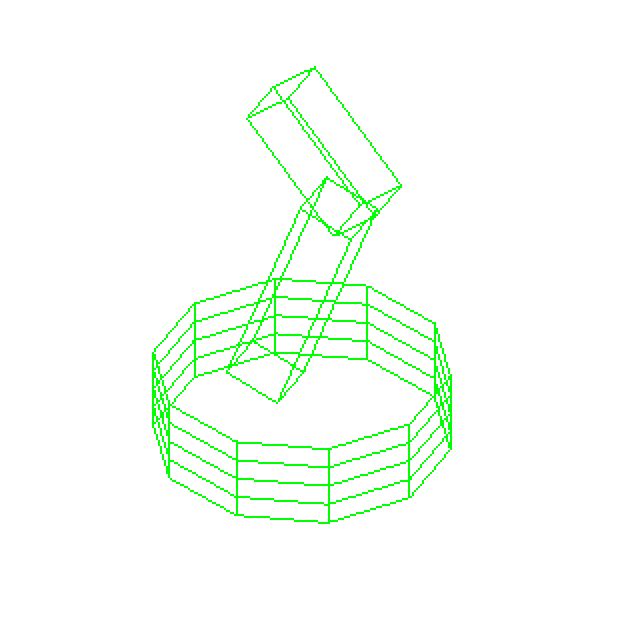
\includegraphics[width=0.5\hsize]{robot.png}
            \caption{アームロボット}
            \label{fig:robot}
        \end{figure}

    \subsection*{4.}
        作成したタイマーコールバック関数をリスト\ref{src:timer}に示す。

        \begin{lstlisting}[caption=タイマーコールバック関数, label=src:timer]
void timer(int dummy) {
    glutTimerFunc(15, timer, 0);

    rotAng[0] += BASE_SPEED;

    rotAng[1] = AMP * sin((double)LOWER_SPEED * rotAng[0] / 180.0 * M_PI);
    rotAng[2] = AMP * sin((double)UPPER_SPEED * rotAng[0] / 180.0 * M_PI);

    glutPostRedisplay();
}\end{lstlisting}
        
        \verb|BASE_SPEED|, \verb|LOWER_SPEED|, \verb|UPPER_SPEED|, \verb|AMP|
        はそれぞれ台座の回転速度、下腕の回転速度、上腕の回転速度、両腕の振幅であり、
        2本の腕が異なる速度で振動する。
        異なる速度で振動させることでアームロボットが踊っているように見えた。

\section*{課題$\rm I\hspace{-.01em}I\hspace{-.01em}I$}
    \subsection*{1.}
        $P_1$から$P_2$のベクトル、$P_1$から$P_3$のベクトルを
        それぞれ$\overrightarrow{P_1P_2}, \overrightarrow{P_1P_3}$とする。
        $\triangle{P_1P_2P_3}$はこの2本のベクトルが成す平面上にあるので、
        その単位法線ベクトルは、
        $\displaystyle\pm\frac{\overrightarrow{P_1P_2}\times\overrightarrow{P_1P_3}}{|\overrightarrow{P_1P_2}\times\overrightarrow{P_1P_3}|}$
        である。

    \subsection*{2.}
        ある点から$P_1, P_2$に向かうベクトルを$v_1, v_2$とすると、$v_1\times v_2$
        の符号でその点が$\triangle P_1P_2P_3$のどちらの面にあるか判断できる。
        
    \subsection*{3.}
        Phongの照光モデルは1975年にユタ大学のBui Tuong Phongによって提案された\cite{phong}。
        このモデルは物体が発する光を環境光、拡散反射光、鏡面反射光の和としている。
        非常に単純で、計算量も小さいため、従来、標準シェーダーとして用いられてきた。
        しかし、近似モデルであるため、大域照明を記述することができない。

    \subsection*{4.}
        頂点の法線ベクトルは、図形の中心からその頂点に向かうベクトルとすれば良い。
        よって、原点を中心とする図形の場合、頂点の位置ベクトルと一致する。
        三つの図形を表示するプログラムの主要部をリスト
        \ref{src:tetrahedron}, \ref{src:cube}, \ref{src:octahedron}、
        三つの図形を\ref{fig:tetrahedron}, \ref{fig:cube}, \ref{fig:octahedron}に示す。

        \begin{lstlisting}[caption=正四面体を表示するプログラム, label=src:tetrahedron]
GLdouble vP[4][3] = {
    { 1.000,  0.000,  0.000},
    {-0.333,  0.943,  0.000},
    {-0.333, -0.471,  0.816},
    {-0.333, -0.471, -0.816}
};
int tP[4][3] = {
    {0, 1, 2},
    {0, 2, 3},
    {0, 3, 1},
    {1, 3, 2}
};

void display() {
    int i,j;
    glClear(GL_COLOR_BUFFER_BIT | GL_DEPTH_BUFFER_BIT);
    glMatrixMode(GL_MODELVIEW);

    glBegin(GL_TRIANGLES);
    for (i = 0; i < 4; i++) {
        for (j = 0; j < 3; j++) {
            glColor3d(0, 0, 0);
            glNormal3dv(vP[tP[i][j]]);
            glVertex3dv(vP[tP[i][j]]);
        }
    }
    glEnd();

    glutSwapBuffers();
}
\end{lstlisting}

        \begin{lstlisting}[caption=正六面体を表示するプログラム, label=src:cube]
GLdouble vP[8][3] = {
    {-0.577, -0.577, 0.577},
    {0.577, -0.577, 0.577},
    {0.577, -0.577, -0.577},
    {-0.577, -0.577, -0.577},
    {-0.577, 0.577, 0.577},
    {0.577, 0.577, 0.577},
    {0.577, 0.577, -0.577},
    {-0.577, 0.577, -0.577}
};
int tP[6][4] = {
    {0, 1, 5, 4},
    {0, 4, 7, 3},
    {1, 2, 6, 5},
    {3, 2, 1, 0},
    {3, 7, 6, 2},
    {4, 5, 6, 7}
};

void display() {
    int i,j;
    glClear(GL_COLOR_BUFFER_BIT | GL_DEPTH_BUFFER_BIT);
    glMatrixMode(GL_MODELVIEW);

    glBegin(GL_QUADS);
    for (i = 0; i < 6; i++) {
        for (j = 0; j < 4; j++) {
            glColor3d(0, 0, 0);
            glNormal3dv(vP[tP[i][j]]);
            glVertex3dv(vP[tP[i][j]]);
        }
    }
    glEnd();

    glutSwapBuffers();
}
\end{lstlisting}

        \begin{lstlisting}[caption=正八面体を表示するプログラム, label=src:octahedron]
GLdouble vP[6][3] = {
    { 1,  0,  0},
    { 0,  1,  0},
    { 0,  0,  1},
    {-1,  0,  0},
    { 0, -1,  0},
    { 0,  0, -1}
};
int tP[8][3] = {
    {0, 1, 2},
    {0, 4, 5},
    {2, 1, 3},
    {2, 4, 0},
    {3, 4, 2},
    {3, 1, 5},
    {5, 1, 0},
    {5, 4, 3}
};

void display() {
    int i,j;
    glClear(GL_COLOR_BUFFER_BIT | GL_DEPTH_BUFFER_BIT);
    glMatrixMode(GL_MODELVIEW);

    glBegin(GL_TRIANGLES);
    for (i = 0; i < 8; i++) {
        for (j = 0; j < 3; j++) {
            glColor3d(0, 0, 0);
            glNormal3dv(vP[tP[i][j]]);
            glVertex3dv(vP[tP[i][j]]);
        }
    }
    glEnd();

    glutSwapBuffers();
}
\end{lstlisting}

        \begin{figure}[h]
            \begin{minipage}{0.33\hsize}
                \centering
                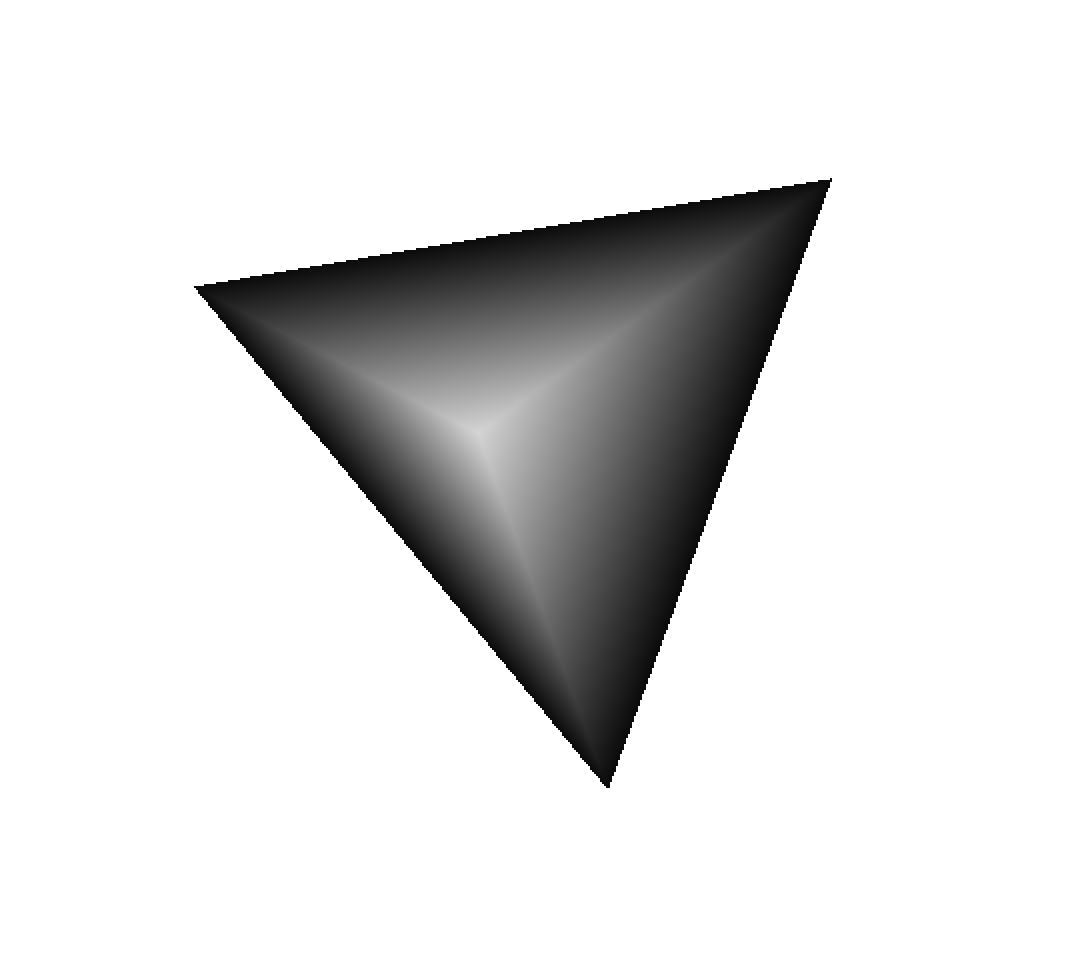
\includegraphics[width=1\hsize]{tetrahedron.png}
                \caption{正四面体}
                \label{fig:tetrahedron}
            \end{minipage}
            \begin{minipage}{0.33\hsize}
                \centering
                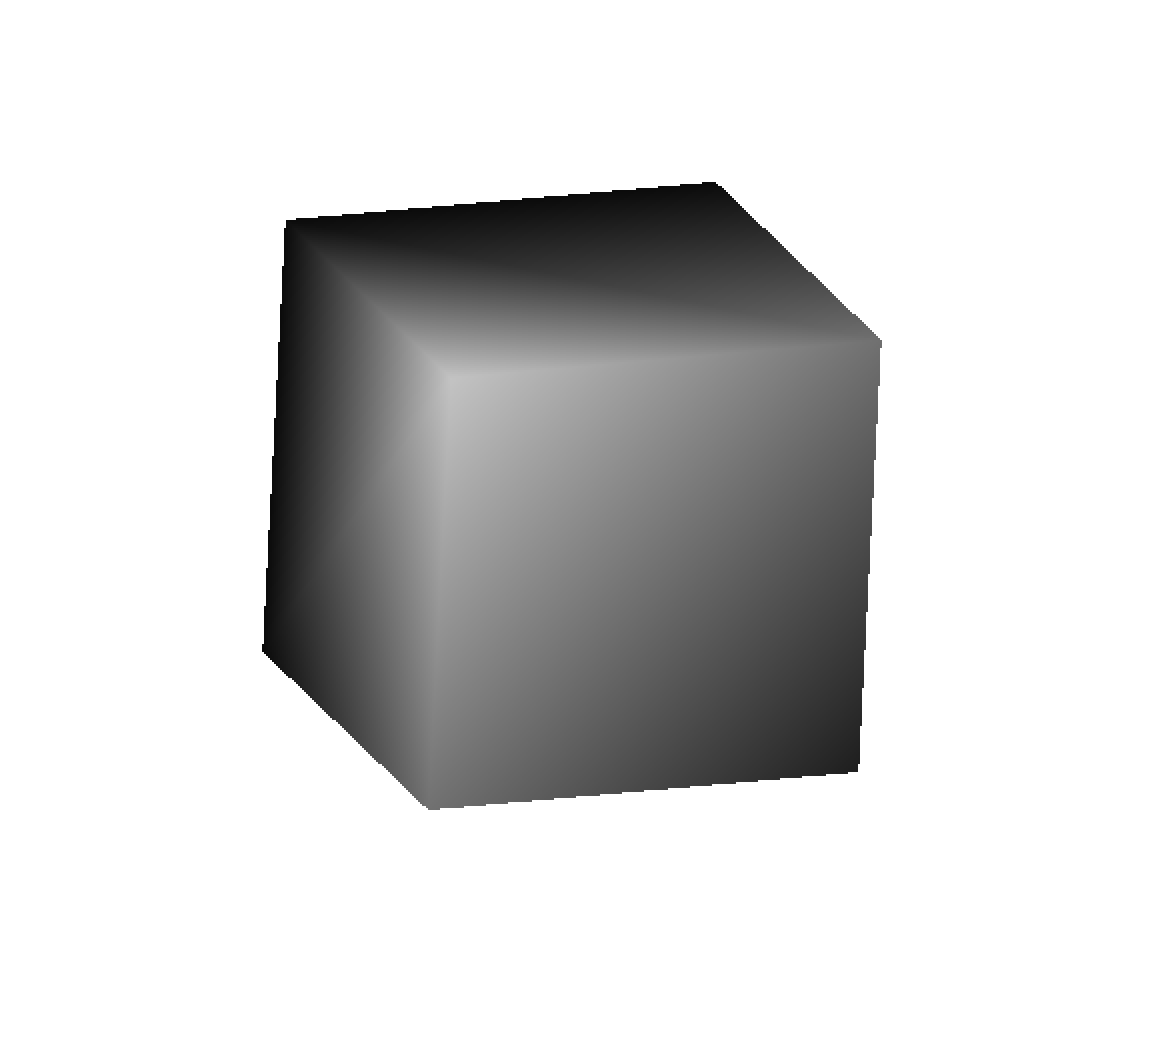
\includegraphics[width=1\hsize]{cube.png}
                \caption{正六面体}
                \label{fig:cube}
            \end{minipage}
            \begin{minipage}{0.33\hsize}
                \centering
                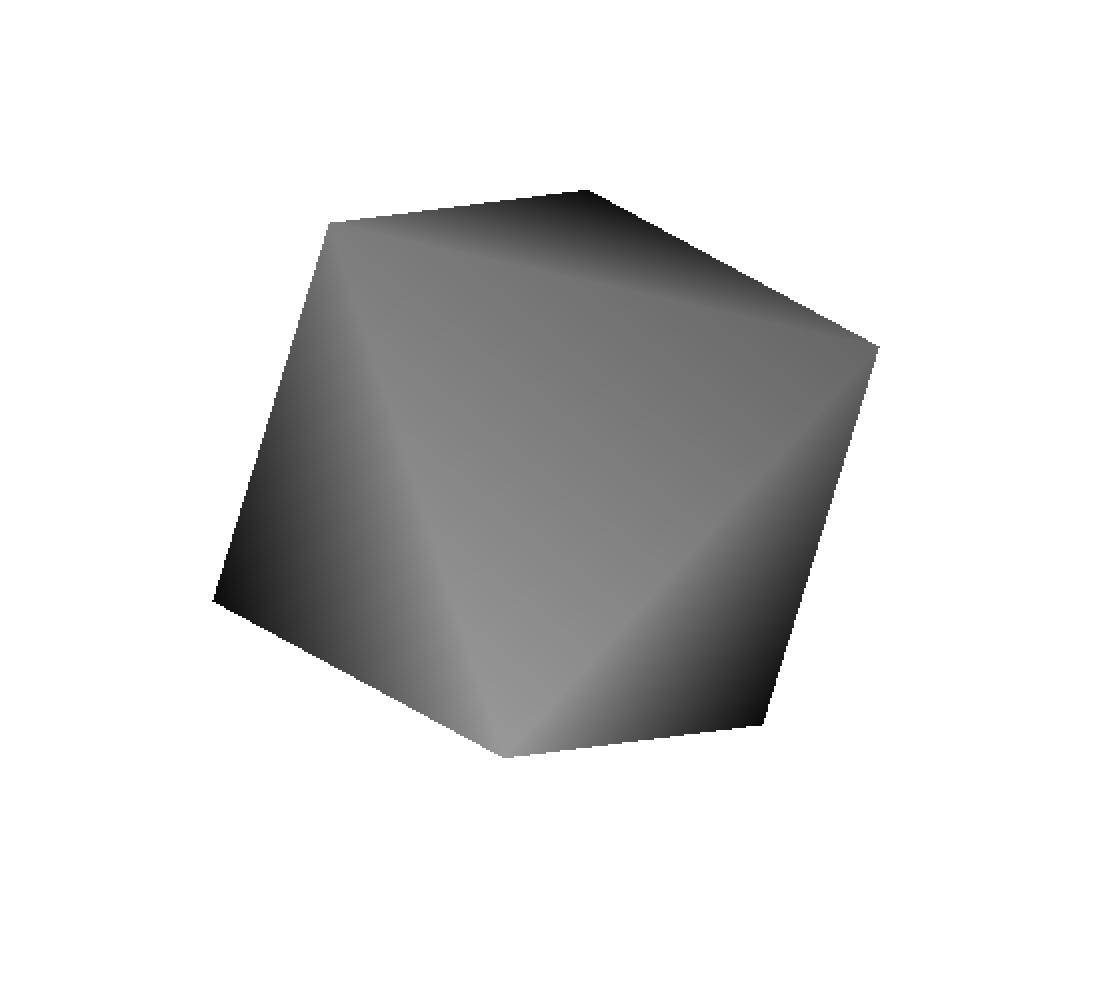
\includegraphics[width=1\hsize]{octahedron.png}
                \caption{正八面体}
                \label{fig:octahedron}
            \end{minipage}
        \end{figure}

    \subsection*{5.}
        図\ref{fig:real}に、シェーディング表示にしたロボットアームを示す。

        \begin{figure}[h]
            \centering
            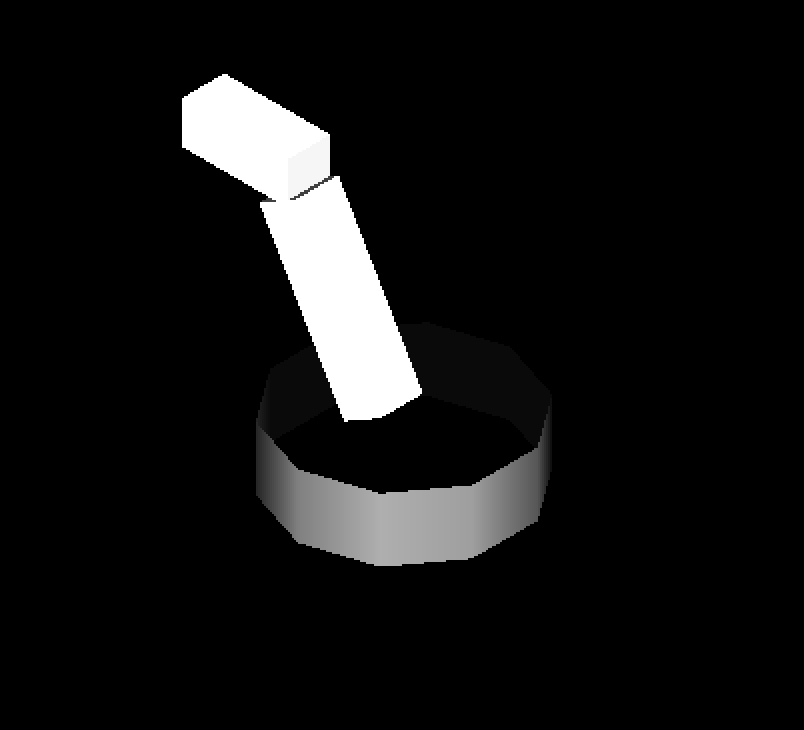
\includegraphics[width=0.5\hsize]{real.png}
            \caption{シェーディング表示のロボットアーム}
            \label{fig:real}
        \end{figure}

\section*{感想等}
    身近なソフトウェアにOpenGLはよく使われているが、実際に自分でOpenGLを
    扱ったことはなかったので、新しい体験ができた。
    OpenGLはあまり直感的にプログラムを書くのが難しく、
    今では当たり前になっているGUIの裏では
    そこそこ面倒なプログラミングがなされていることを知った。

    テキストの改善点として、課題の設問文が少しわかりづらい点をあげる。
    特に課題IIIの2など、
    どのような条件で具体的に何を求めれば良いかがわかりづらかった。

\begin{thebibliography}{99}
    \bibitem{grep}{
        ``grepコマンド'', IBM, https://www.ibm.com/docs/ja/aix/7.1?topic=grep-command, 2020
    }
    \bibitem{text}{
        ``R03-Ec5 プログラミング演習$\rm I\hspace{-.01em}I$テキスト'',
        高橋章, 2021
    }
    \bibitem{touch}{
        ``touchコマンド'', IBM, https://www.ibm.com/docs/ja/aix/7.1?topic=t-touch-command, 2020
    }
    \bibitem{phong}{
        ``Illumination for computer generated pictures'',
        Bui Tuong Phong, Communications of the ACM vol. 18, 311-317,
        1975
    }
\end{thebibliography}
\end{document}